\documentclass[10pt,twocolumn,letterpaper]{article}

\usepackage{cvpr}
\usepackage{times}
\usepackage{epsfig}
\usepackage{graphicx}
\usepackage{amsmath}
\usepackage{amssymb}
\usepackage{amsfonts}       % blackboard math symbols
%\usepackage{nicefrac}       % compact symbols for 1/2, etc.
%\usepackage{microtype}      % microtypography

\usepackage{url}
\usepackage[table]{xcolor}
\usepackage{bbm}
\usepackage{booktabs}
\usepackage[T1]{fontenc}
\usepackage{fix-cm}
\usepackage{array}
\usepackage{epsfig}
%\usepackage{mathabx}
%\usepackage{dsfont}
\usepackage{multirow}

\usepackage{times}
\usepackage{helvet}
\usepackage{courier}
\usepackage{graphicx}
\usepackage{bm}
\usepackage{color}
\usepackage{epstopdf}
\usepackage{caption}
\usepackage{subcaption}
\usepackage{enumitem}
\usepackage{calc}
\usepackage{multirow}
\usepackage{xspace}
\usepackage{booktabs}
\usepackage{mathrsfs}
\usepackage{array}
\usepackage{gensymb}

% Include other packages here, before hyperref.

% If you comment hyperref and then uncomment it, you should delete
% egpaper.aux before re-running latex.  (Or just hit 'q' on the first latex
% run, let it finish, and you should be clear).
\usepackage[pagebackref=true,breaklinks=true,letterpaper=true,colorlinks,bookmarks=false]{hyperref}
\usepackage{caption}
\captionsetup{skip=3pt}

\cvprfinalcopy % *** Uncomment this line for the final submission
\newcommand{\figref}[1]{Fig\onedot~\ref{#1}}
\newcommand{\equref}[1]{Eq\onedot~\eqref{#1}}
\newcommand{\secref}[1]{Sec\onedot~\ref{#1}}
\newcommand{\tabref}[1]{Tab\onedot~\ref{#1}}
\newcommand{\thmref}[1]{Theorem~\ref{#1}}
\newcommand{\prgref}[1]{Program~\ref{#1}}
\newcommand{\algref}[1]{Alg\onedot~\ref{#1}}
\newcommand{\clmref}[1]{Claim~\ref{#1}}
\newcommand{\lemref}[1]{Lemma~\ref{#1}}
\newcommand{\ptyref}[1]{Property\onedot~\ref{#1}}

\newcommand{\ve}[1]{{\mathbf #1}} % for displaying a vector or matrix
\newcommand*\rot[1]{\rotatebox{45}{#1}}
\newcommand{\hua}[1]{{\mathcal #1}}
\newcommand{\scr}[1]{{\mathcal #1}}
\newcommand{\by}[2]{\ensuremath{#1 \! \times \! #2}}

%\makeatletter
\DeclareRobustCommand\onedot{\futurelet\@let@token\@onedot}
\def\onedot{\ifx\@let@token.\else.\null\fi\xspace}
\def\eg{\emph{e.g.}}
\def\Eg{\emph{E.g}\onedot}
\def\any{\forall}
\def\ie{\emph{i.e.}}
\def\Ie{\emph{I.e}\onedot}
\def\cf{\emph{cf}\onedot}
\def\Cf{\emph{Cf}\onedot}
\def\etc{\emph{etc}\onedot}
\def\vs{\emph{vs}\onedot}
\def\wrt{w.r.t\onedot}
\def\dof{d.o.f\onedot}
\def\etal{\emph{et al.}}

\def\cvprPaperID{936} % *** Enter the CVPR Paper ID here
\def\httilde{\mbox{\tt\raisebox{-.5ex}{\symbol{126}}}}

% Pages are numbered in submission mode, and unnumbered in camera-ready
\ifcvprfinal\pagestyle{empty}\fi
\begin{document}

%%%%%%%%% TITLE
\onecolumn
\title{DeLS-3D: Deep Localization and Segmentation with a 3D Semantic Map -- Supplementary Materials}
\maketitle
%\thispagestyle{empty}

%%%%%%%%% ABSTRACT
\begin{itemize}
\vspace{-0.5\baselineskip}
    \setlength{\itemsep}{-2pt}
    \item Video of labeled Zpark dataset, \ie images, labeled 3D semantic maps, camera pose inside and semantic labels of each frame.
    \item Video of localization and parsing results over the Zpark dataset, \ie rendered label map with simulated noisy pose, rectified pose after pose RNN and parsing results with the approach.
\vspace{-0.4\baselineskip}
\end{itemize}

Due to the limitation of upload size, we can not upload full-size videos. Thus, we uploaded low resolution videos for reviewers to briefly check the results. 
Additionally, we upload the original videos of dataset and results to YouTube and Baidu Cloud for better visualization. Here, we illustrate a snapshot for each of the videos to clearify their meaning.

\section{Dataset} 
Youtube link~\url{https://www.youtube.com/watch?v=z7vcOHK74zY}

Baidu Cloud~\url{https://pan.baidu.com/s/1jHC1cmq}

\begin{figure*}[!hbpt]
\center
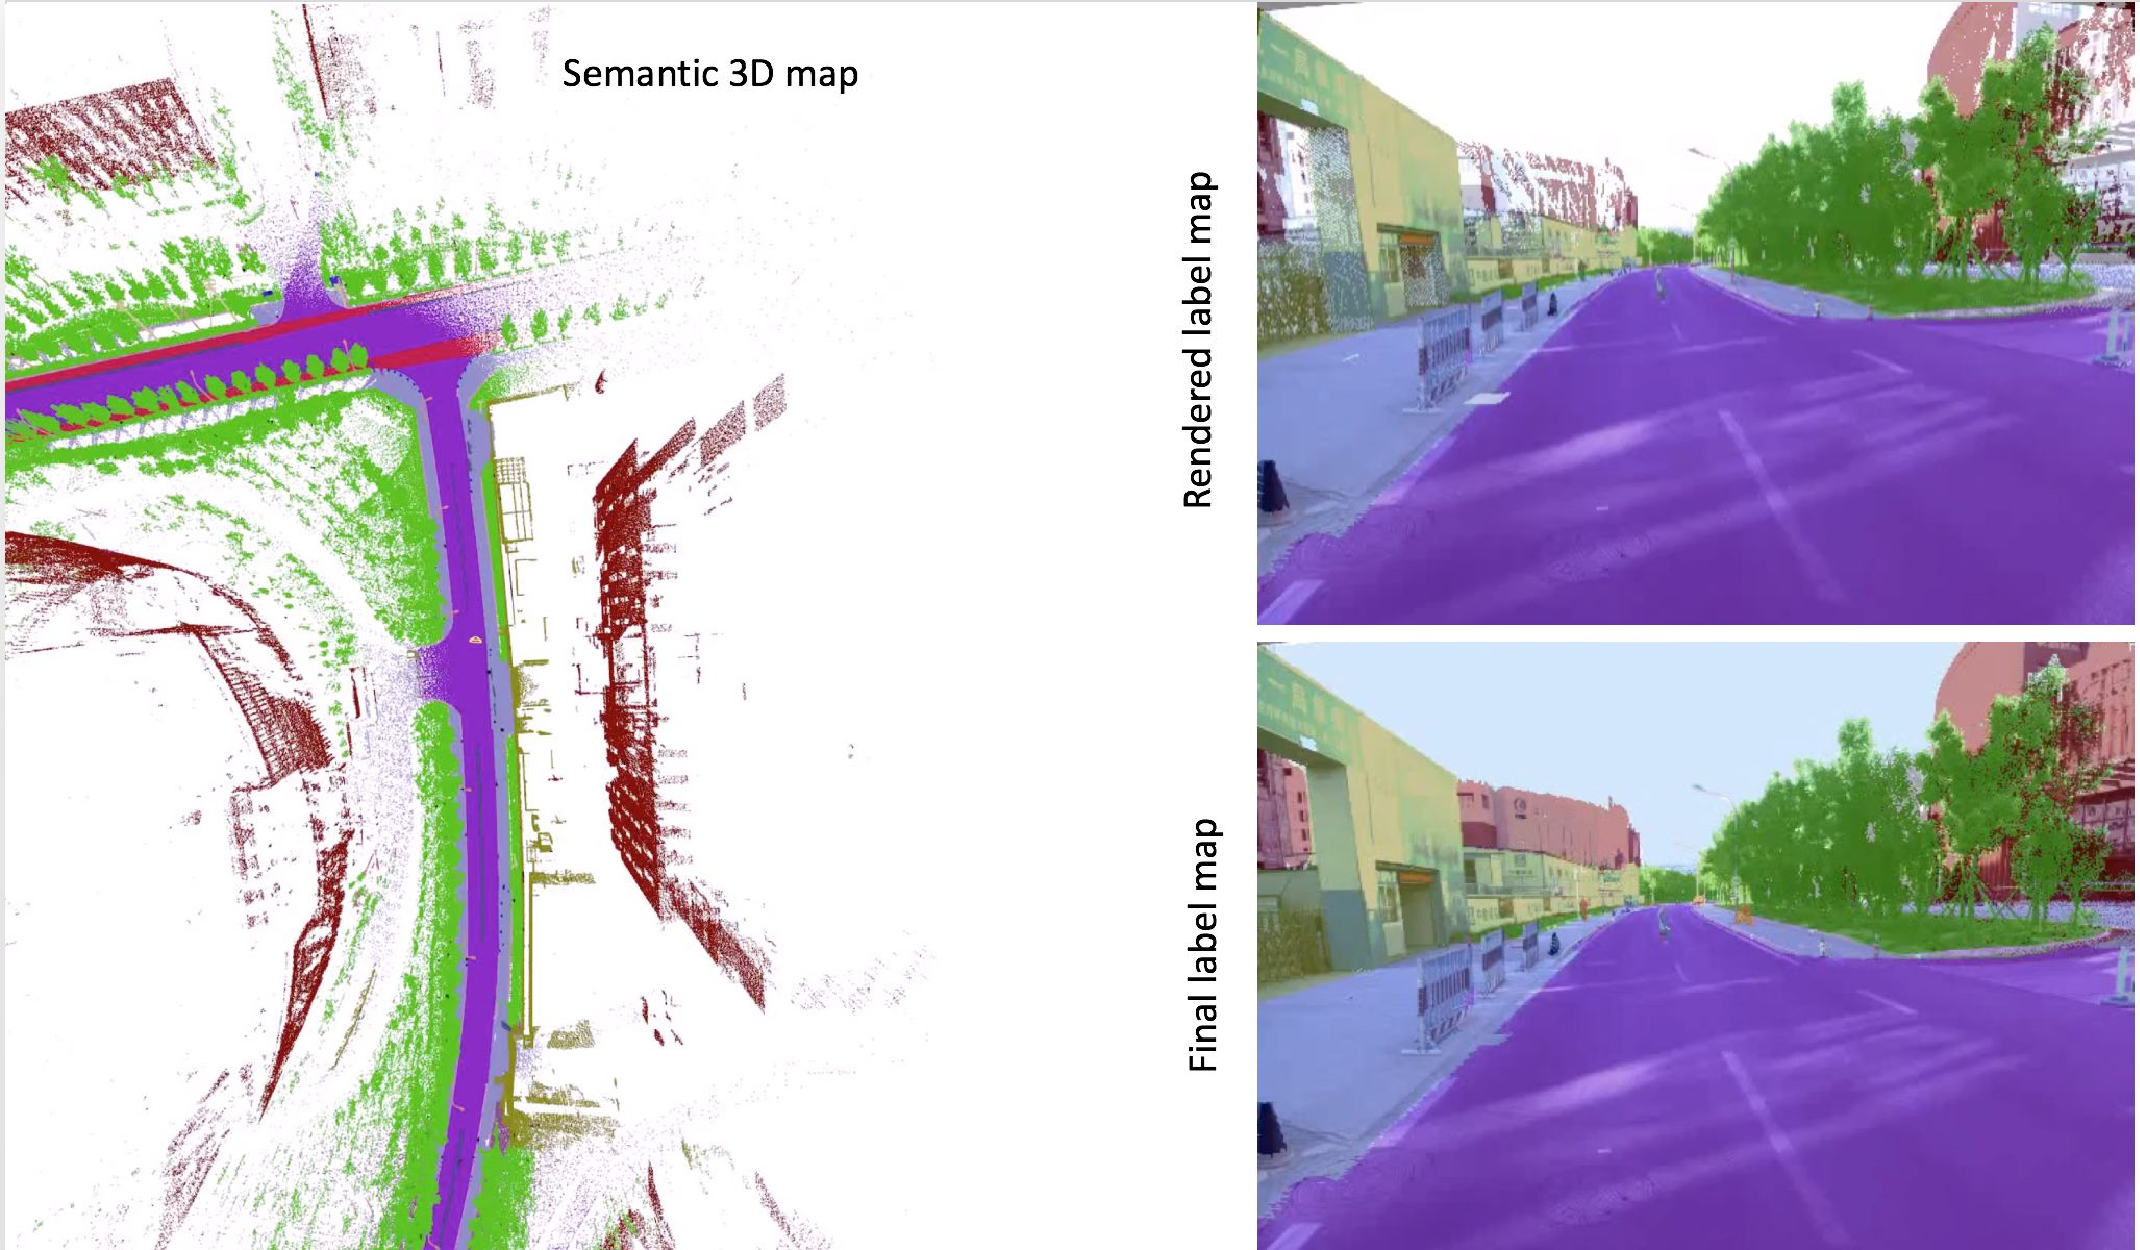
\includegraphics[width=0.9\textwidth]{fig/dataset_video.pdf}
\caption{Zpark dataset overview. Left pane: the bird's eye view of our 3D map. Right top: the rendered label map from 3D with ground truth pose. Right bottom: the manually labeled map. Check video for the full content.}
\label{fig:framework}
\end{figure*}


\section{Results} 
Here we upload part of the results video online. Our full results will be released jointly with the datasets.

\paragraph{Results for Zpark dataset.}

Youtube link~\url{https://www.youtube.com/watch?v=fqglYBipNfQ}
Baidu Cloud~\url{https://pan.baidu.com/s/1qYPwqgG}

\paragraph{Results for Dlake dataset.} 
Youtube link~\url{https://www.youtube.com/watch?v=fqglYBipNfQ}



\begin{figure*}[!hbpt]
\center
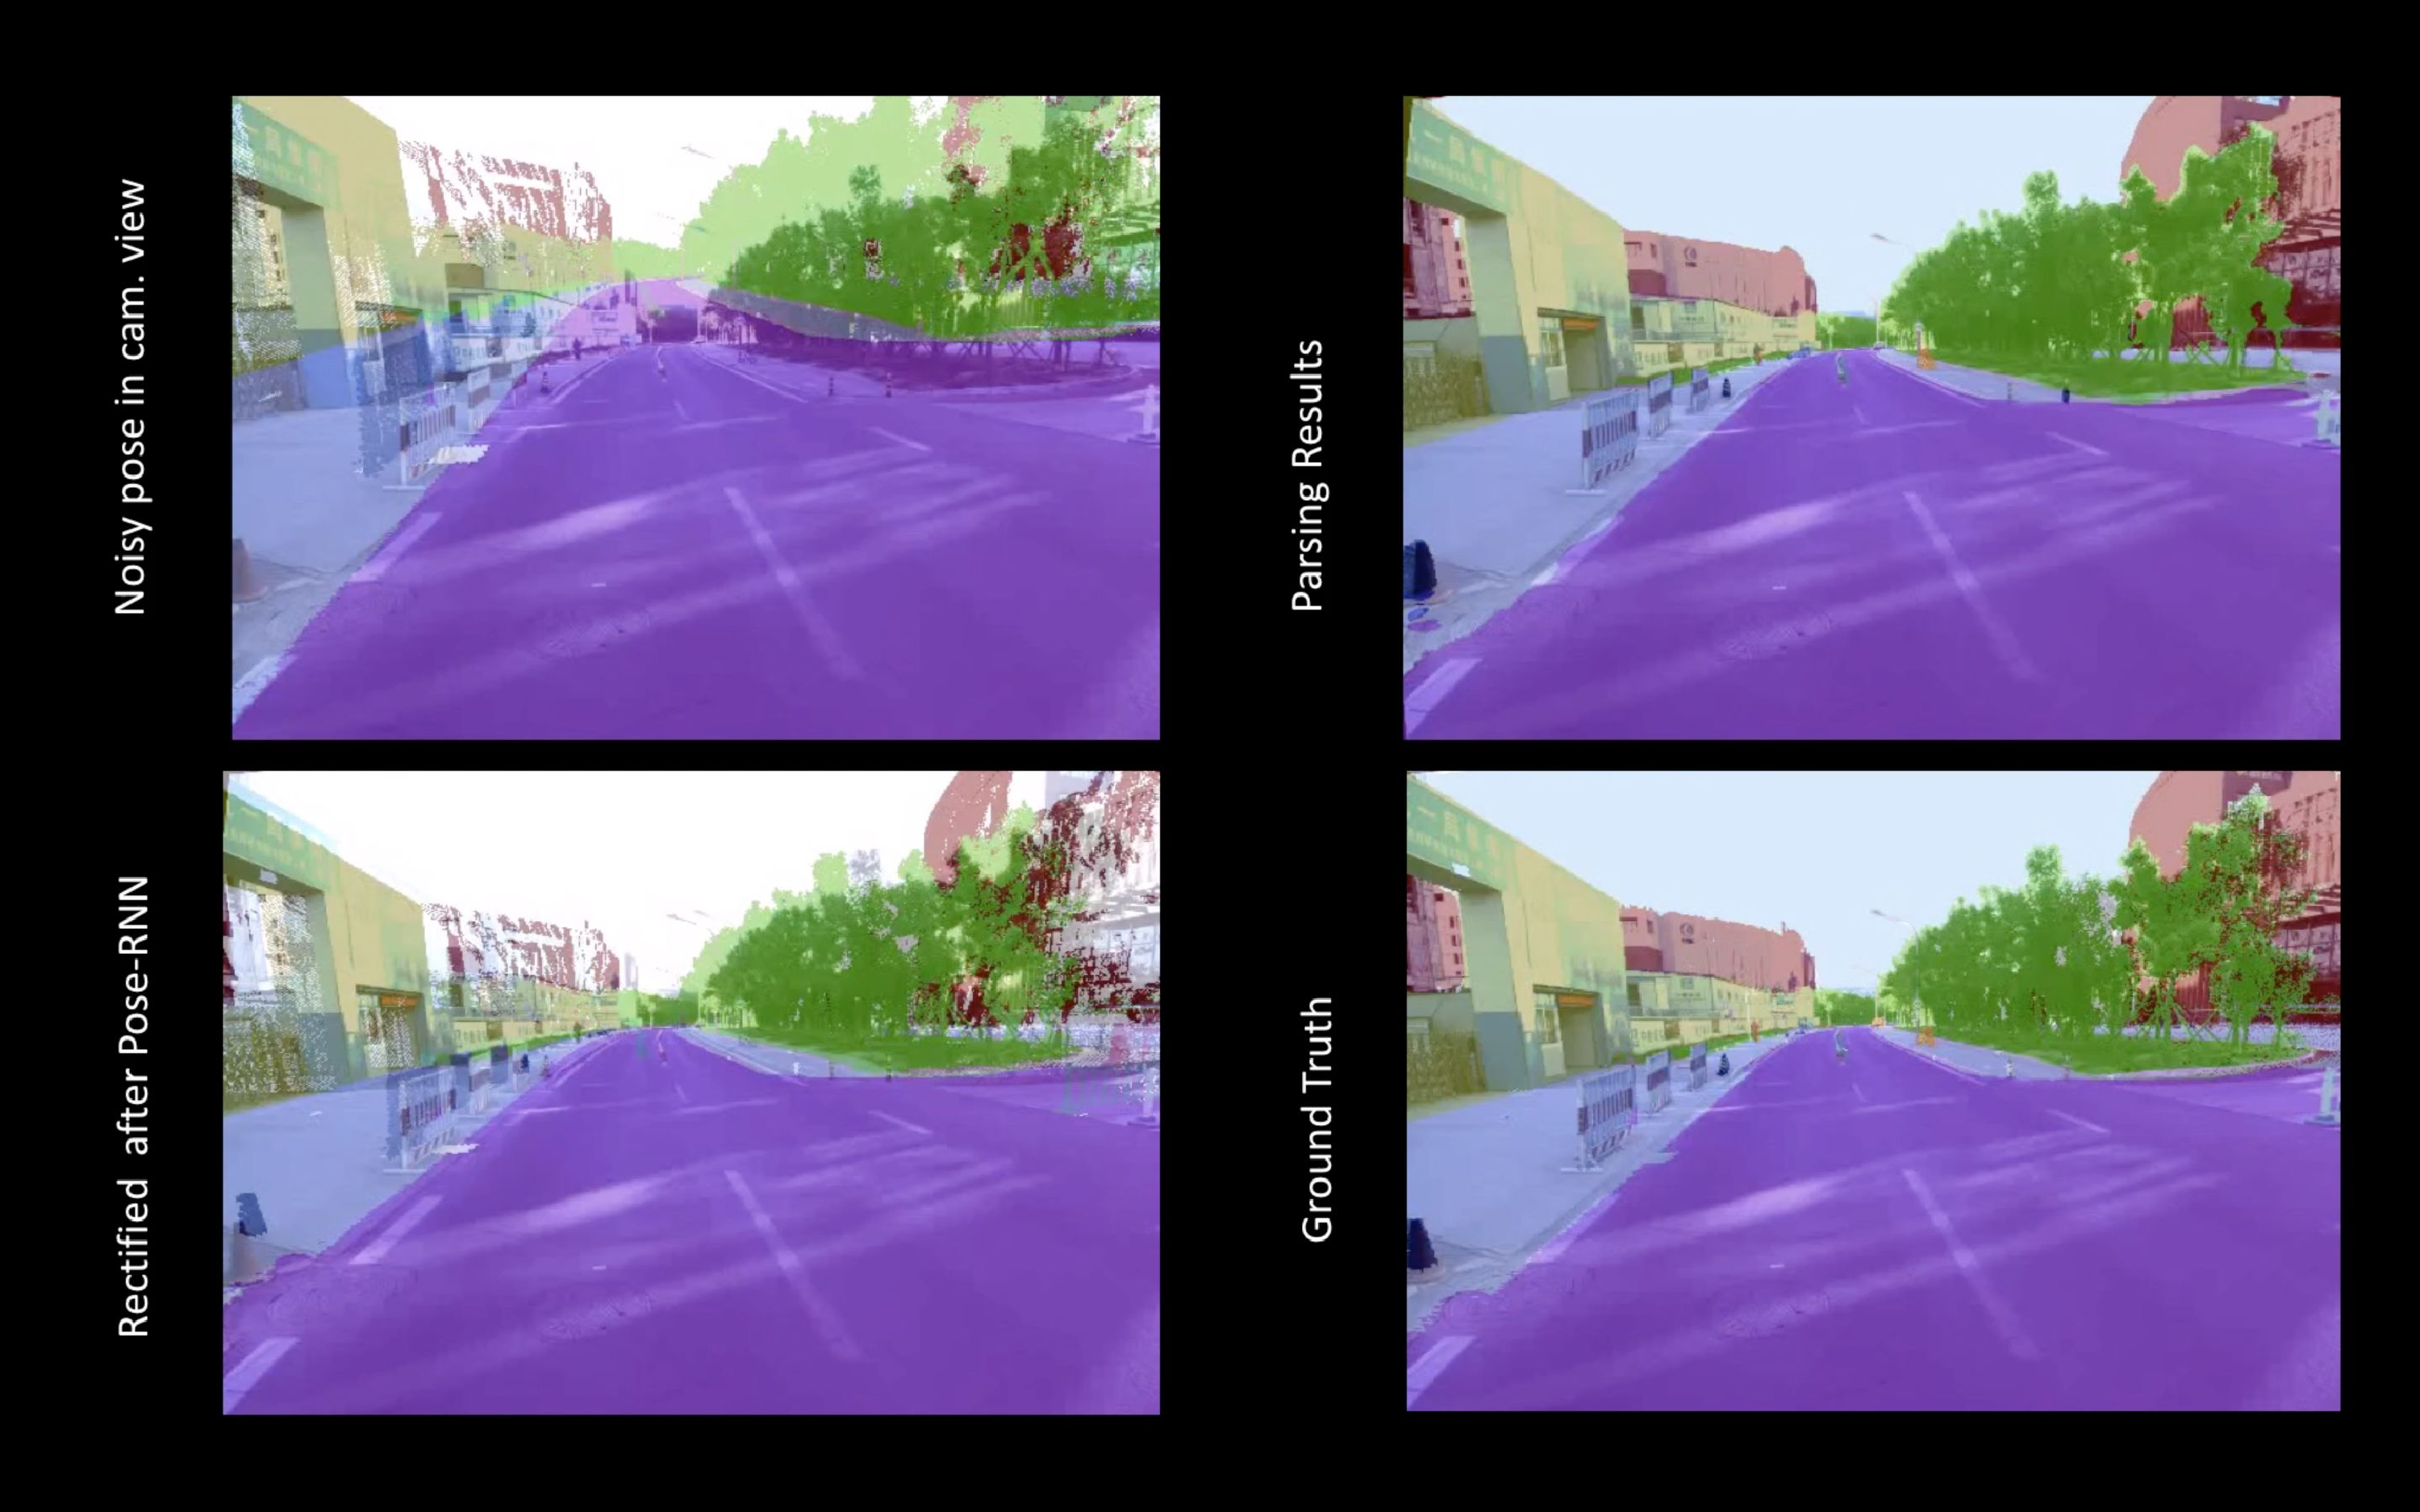
\includegraphics[width=0.8\textwidth]{fig/results_video.pdf}
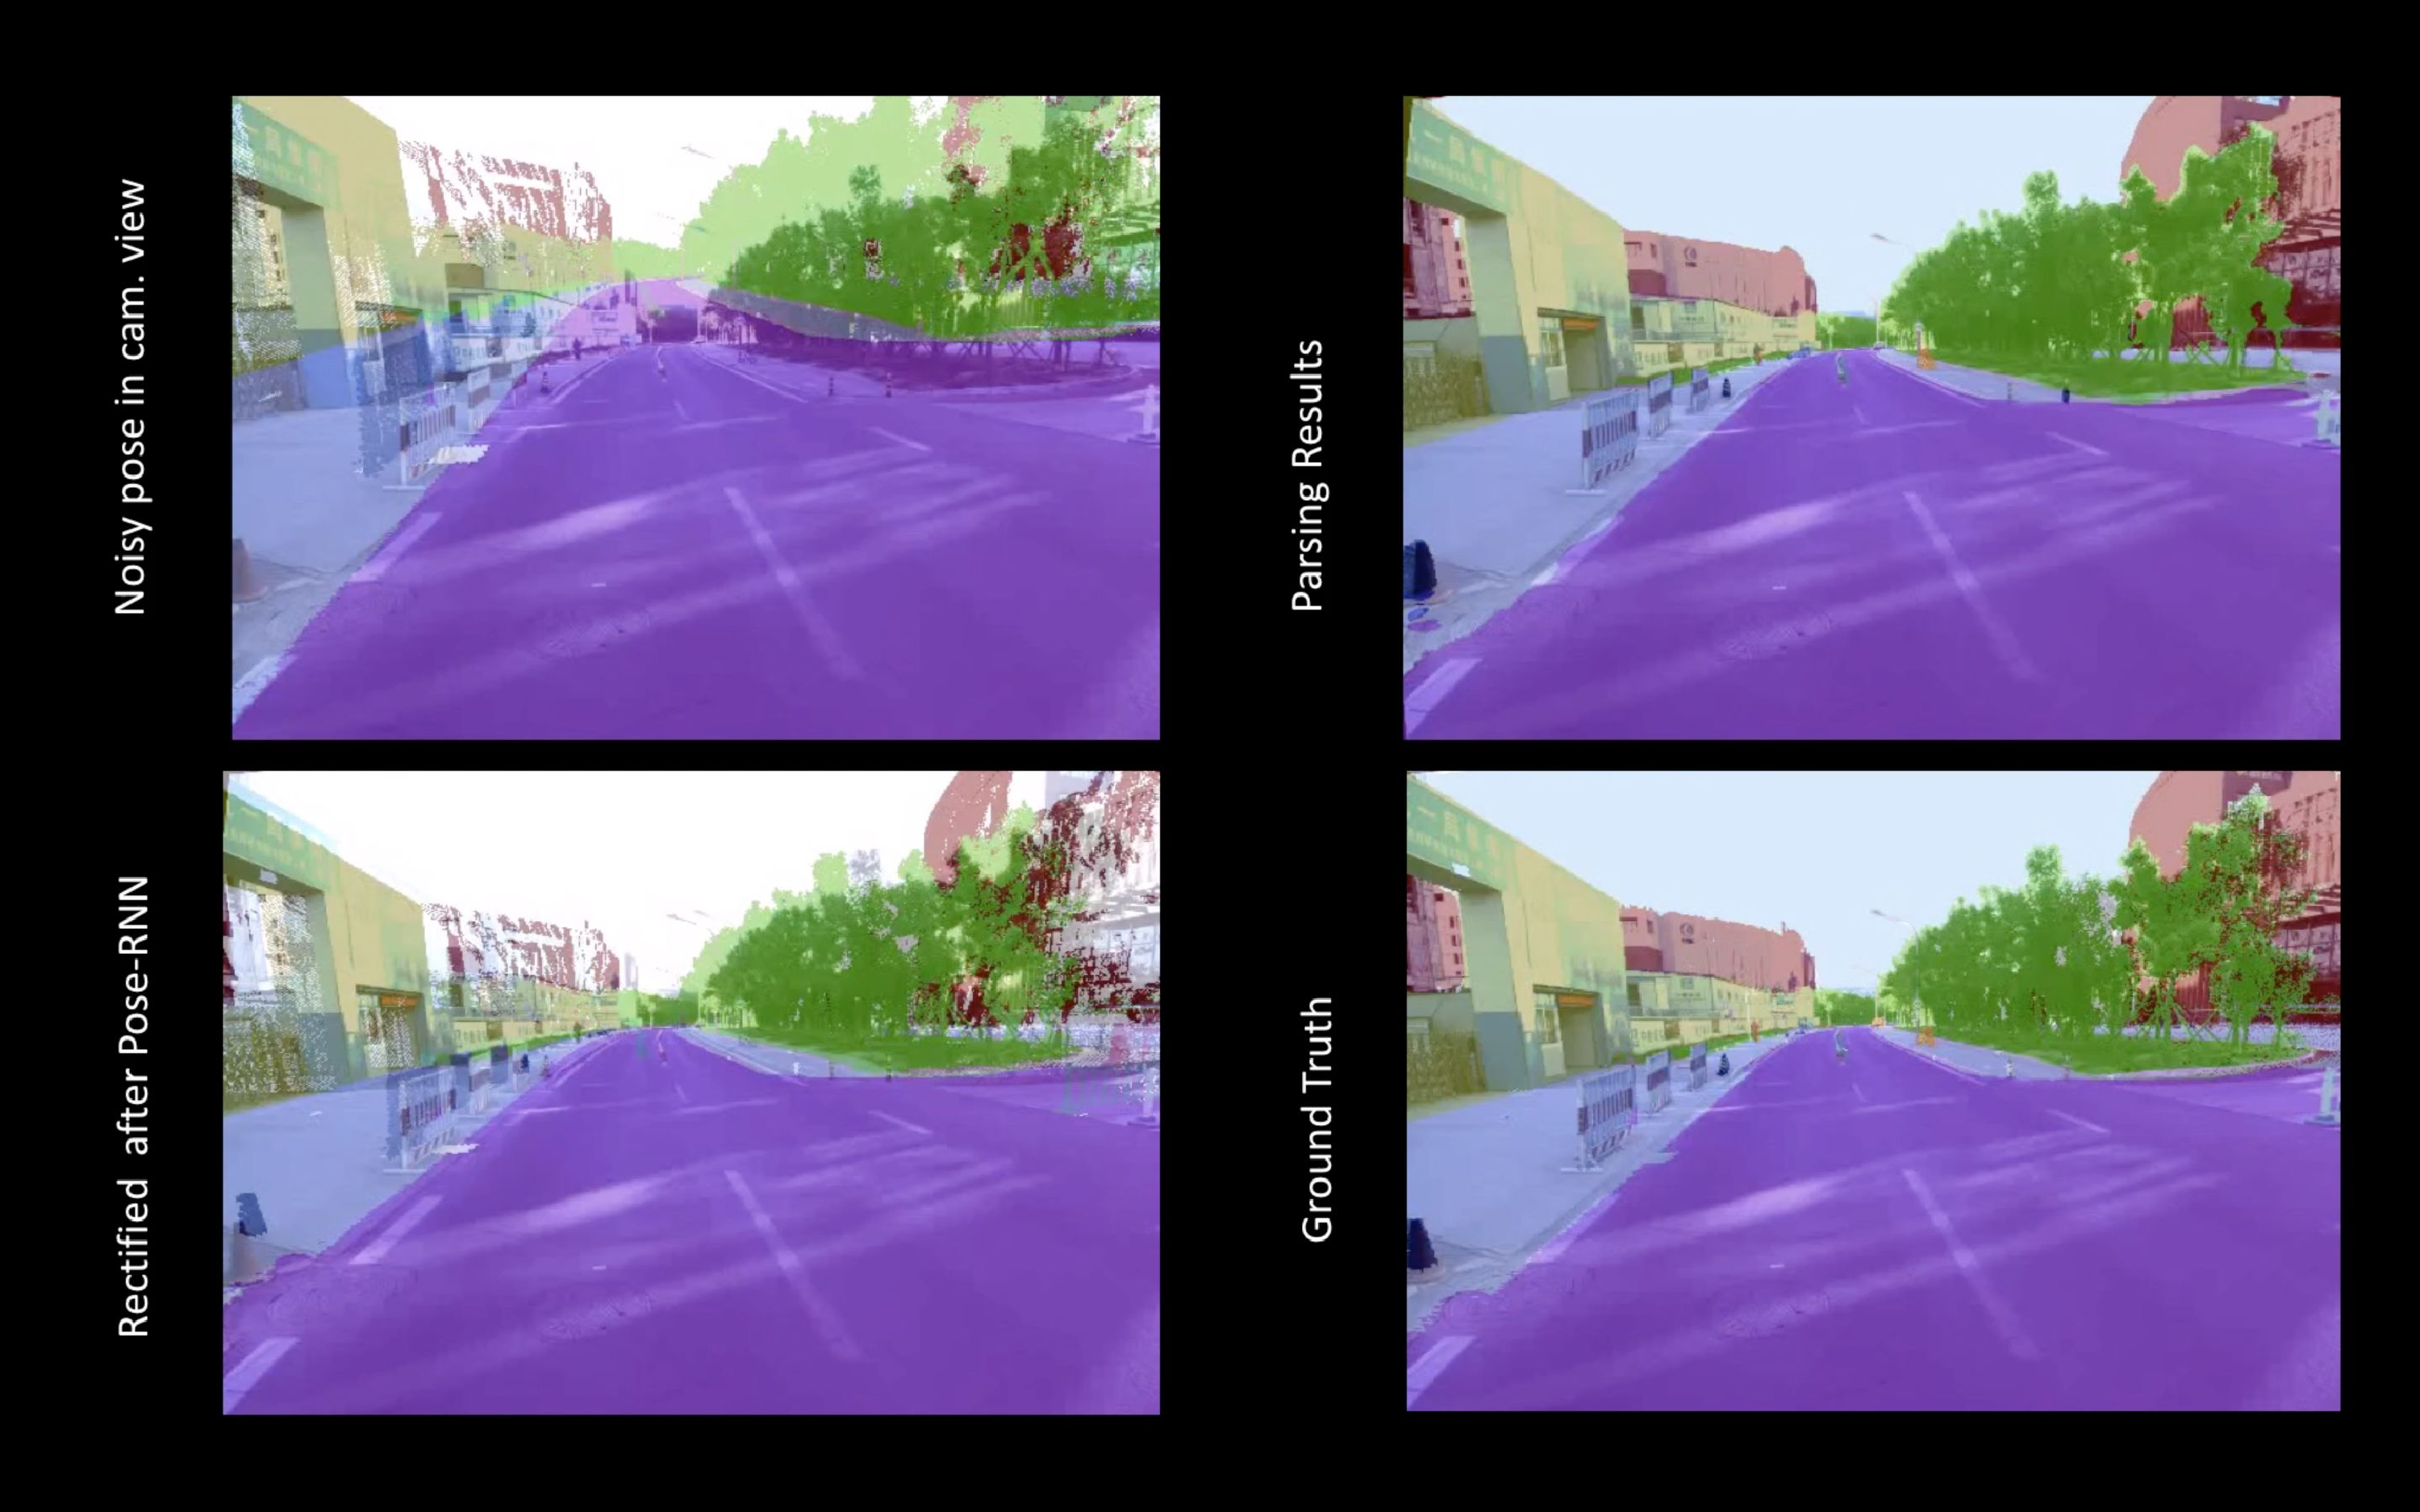
\includegraphics[width=0.8\textwidth]{fig/results_video.pdf}
\caption{The results of a driving video in Zpark dataset (top) and in Dlake dataset (bottom). Left top: the rendered label map with noisy poses. Left bottom: the rendered label map from rectified poses. Right top: the parsing results. Right bottom: ground truth labeled map. Check the video online for the full content.}
\label{fig:framework}
\end{figure*}

% {\small
% \bibliographystyle{ieee}
% \bibliography{egbib}
% }

\end{document}
